\documentclass[11pt,letterpaper]{article}

% Load some basic packages that are useful to have
% and that should be part of any LaTeX installation.
%
% be able to include figures
\usepackage{graphicx}
% get nice colors
\usepackage{xcolor}

% change default font to Palatino (looks nicer!)
\usepackage[latin1]{inputenc}
\usepackage{mathpazo}
\usepackage[T1]{fontenc}
% load some useful math symbols/fonts
\usepackage{latexsym,amsfonts,amsmath,amssymb}

% comfort package to easily set margins
\usepackage[top=1in, bottom=1in, left=1in, right=1in]{geometry}

% control some spacings
%
% spacing after a paragraph
\setlength{\parskip}{.15cm}
% indentation at the top of a new paragraph
\setlength{\parindent}{0.0cm}


\begin{document}

\begin{center}
\Large
Newtonian Binary Coalescence
Ay190 -- Final Project\\
Cutter Coryell and John Pharo\\
Date: \today
\end{center}

\section{Introduction}

The paper \textit{Gravitational Radiation and the Motion of Two Point Masses} (Peters 1964), the equations of general relativity are used to obtain equations of conservation of energy, momentum, and angular momentum. From this, Peters determines the energy loss and angular momentum loss of a binary system of compact objects due to radiating gravitational waves. This yields the equations

$$ \frac{dE}{dt} = \frac{G}{5c^5} \left( \frac{\partial^3 \bar{I}_{ij}}{\partial t^3} \right)^2 \hspace*{.5in} \frac{dL_z}{dt} = \frac{2G}{5c^5} \epsilon_{zjk} \left( \frac{\partial^3 \bar{I}_{ij}}{\partial t^3} \frac{\partial^3 \bar{I}_{km}}{\partial t^3} \right) $$

where $\bar{I}$ is the reduced quadrupole tensor (with separation vector $\vec{x} (t)$ and reduced mass $\mu$):

$$ \bar{I}_{ij}  =\mu (x_i x_j - \frac{1}{3} \delta_{ij} x_k x_k) $$

The purpose of this project is to simulate the orbit and gravitational wave production of such a binary system. This can be done through numerical evaluation of the eccentricity and semi-major axis of the system. Derived in Peters Equations 5.6 and 5.7:

$$ \left< \frac{de}{dt} \right> = - \frac{304}{15} \cdot e \cdot \frac{G^3 m_1 m_2 (m_1 + m_2)}{c^5 a^4 (1 - e^2)^{5/2}} \left( 1 + \frac{121}{304}e^2 \right) $$

$$ \left< \frac{da}{de} \right> = \frac{12}{19} \cdot \frac{a}{e} \cdot \frac{[1 + (73/24)e^2 + (37/96)e^4]}{(1 - e^2)[1 + (121/304)e^2]} $$

Furthermore, we may derive the true anomaly $\varphi$:

$$ \frac{d \varphi}{dt} = \frac{L}{r^2}, \hspace*{.3in} e = \sqrt{1 + \frac{2EL^2}{(GM)^2}} \implies \frac{d \varphi}{dt} = \frac{\sqrt{GMa(1 - e^2)}}{r^2} $$

Through the use of Runge-Kutta integration, we may numerically evaluate these three derivatives in order to track the orbit of the system over time. Furthermore, by updating the separation vector, one can track the change in the reduced quadrupole over time, which the gravitational wave strain:

$$ h_+ = \frac{1}{r} \left( \ddot{\bar{I}}_{xx} - \ddot{\bar{I}}_{yy} \right) \hspace*{.5in} h_{\times} = \frac{2}{r} \ddot{\bar{I}}_{xy} $$

\section{The Code}

This project uses two main sections of code, one for the actual simulation of the binary coalescence and one for analysis and production of plots of the data.

\subsection{Simulation}

The simulation code \textit{simulate.py} is responsible for finding the numerical solutions for the binary system and generating the simulated orbits and gravitational waves produced over a given time scale. \\

The first section of the code sets various constants and parameters for the system. This includes the initial data settings for simulating the Hulse-Taylor binary and several important parameters for running the simulation. Of particular importance here are the names of the input and output directories (depending on whether a simulation is being continued), the ending time for the simulation, and the number of points used in the simulation (these two generate the time grid). \\

The next two sections are a series of helper functions and the main code body itself. The main code begins by either opening a previous simulation to continue where it left off, or by establishing a new set of initial conditions for a new simulation. This done, the code enters the main loop of the program, which will terminate upon reaching the end of the established number of points. Every specified number of iterations, the loop prints an update on its progress. \\

First, the loop calls a helper function to perform RK4 integration on $a$, $e$, and $\varphi$. The RK4 integrator itself uses several helper functions, each representing the right-hand side of the equations presented in the Introduction. Having calculated the values of $a$, $e$, and $\varphi$ at the current time, the code then calls helper functions to calculate the new separation vector and reduced quadrupole tensor, and from these it calculates the wave strain. \\

The code can be set to produce a 3-D display of the orbit as it is calculated; if so, it is at this point in the code that the plot updates. However, it should be noted that running the display slows the simulation down significantly. After this, the loop writes the newly generated data to the appropriate output directory. 

\subsection{Analysis}

The analysis code \textit{analyze.py} is responsible for taking the output generated by the simulation and plotting it in a useful fashion. The first section sets general useful constants in CGS. The second section takes important parameters for analyzing the simulation data, especially the name of the directory containing the data to be analyzed and the number of iterations it contains. \\

The next to sections load the existing data into lists and then use it to calculate the z-component of the orbital angular momentum and the total mechanical energy of the system, using the following equations:

$$ L_z = \sqrt{GMa (1 - e^2)} \hspace*{.5in} E = \frac{1}{2} \left( \frac{GM}{L_z} \right)^2 (e^2 - 1) $$

Finally, the code generates plots of the semi-major axis, eccentricity, energy, and angular momentum versus time and saves the figures to a new output directory. In order to make pyplot plots intelligible, sometimes the data lists are converted to reduced units. This should be made clear in the captions of the plots.

\section{Test and Results}

\subsection{Output4}

\begin{figure}[bth]
\centering
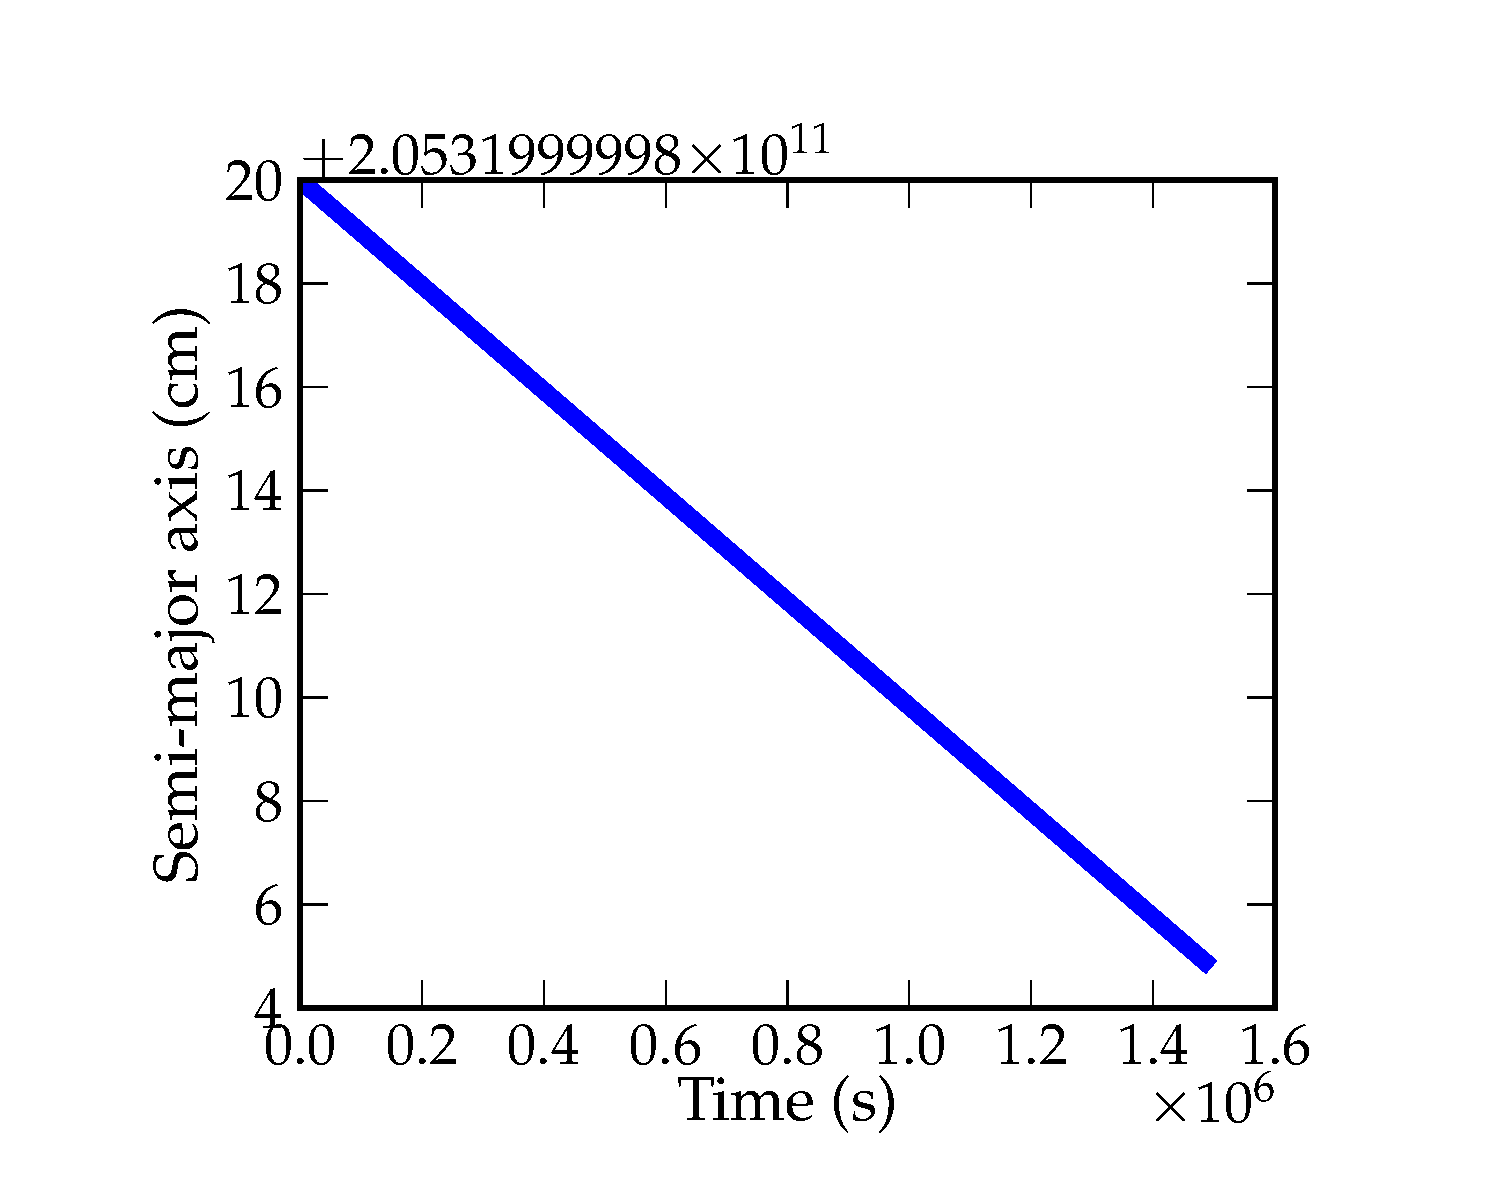
\includegraphics[width=0.5\textwidth]{output4_figs/semi-major_axis.pdf}
\caption{This is the plot of $a$ as a function of time.}
\label{fig:simpleplot2}
\end{figure}

\begin{figure}[bth]
\centering
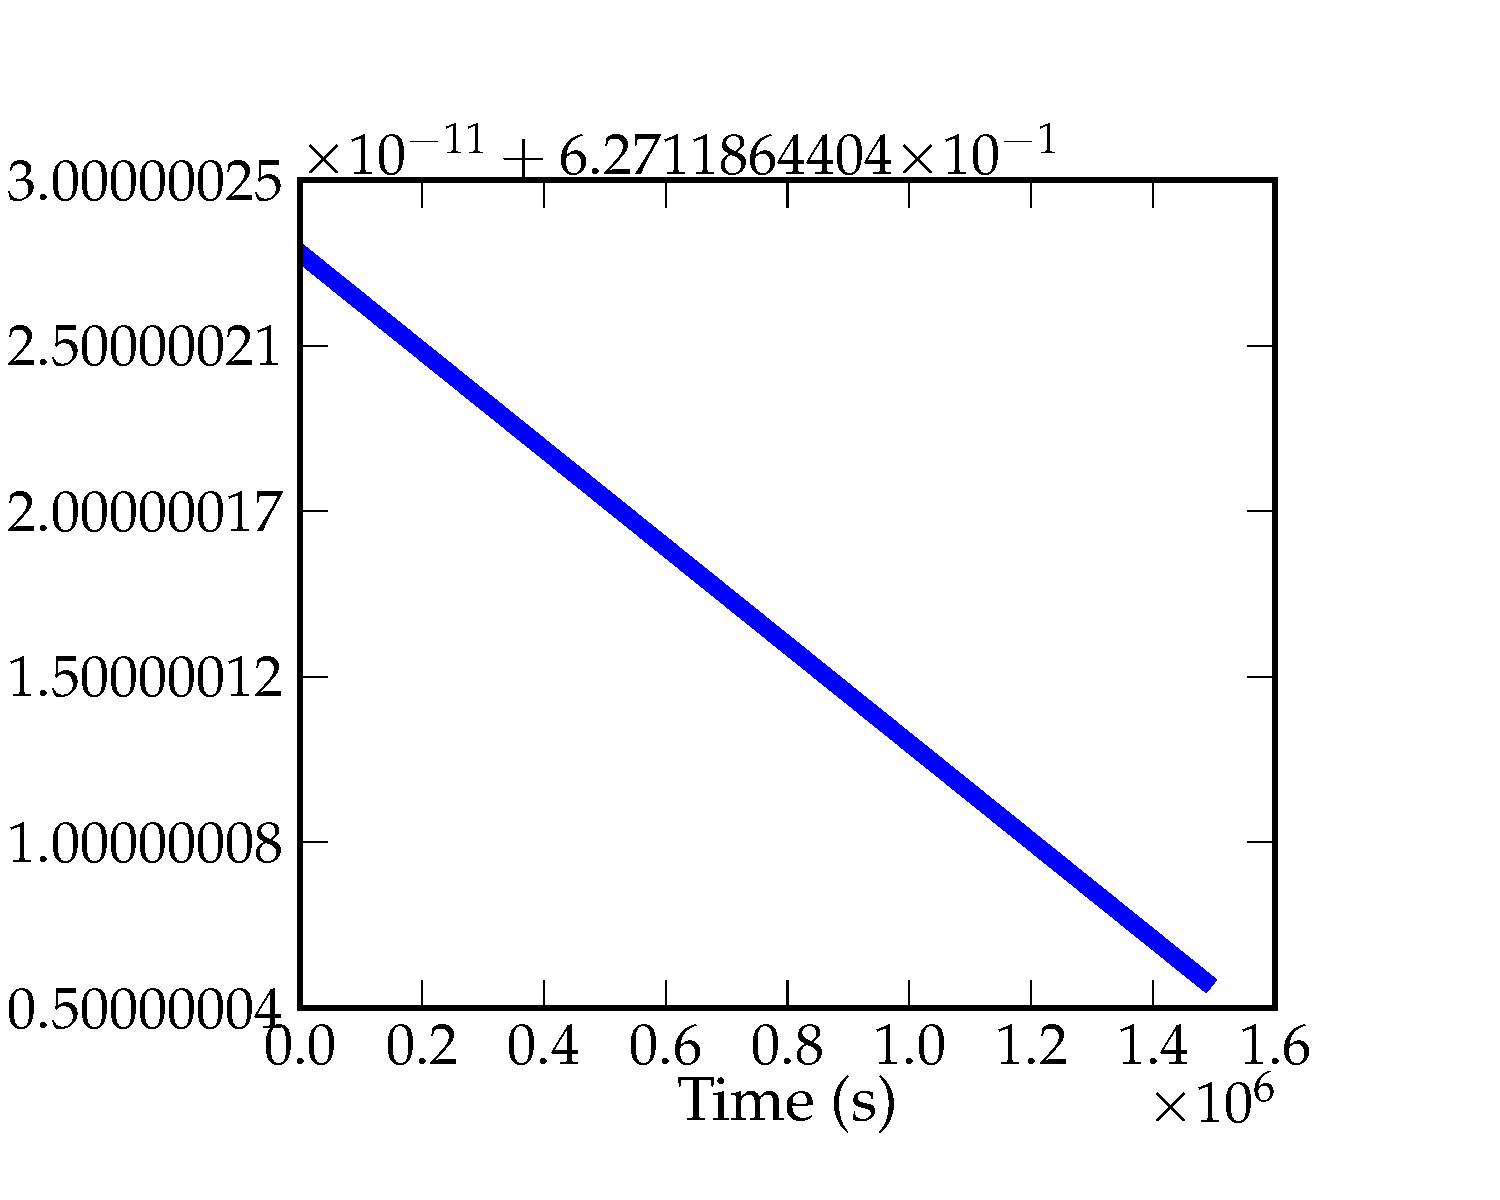
\includegraphics[width=0.5\textwidth]{output4_figs/eccentricity.pdf}
\caption{This is the plot of $e$ as a function of time. This is in reduced units; to get to the actual value of $e$, divide by $10^{10}$.}
\label{fig:simpleplot2}
\end{figure}

\begin{figure}[bth]
\centering
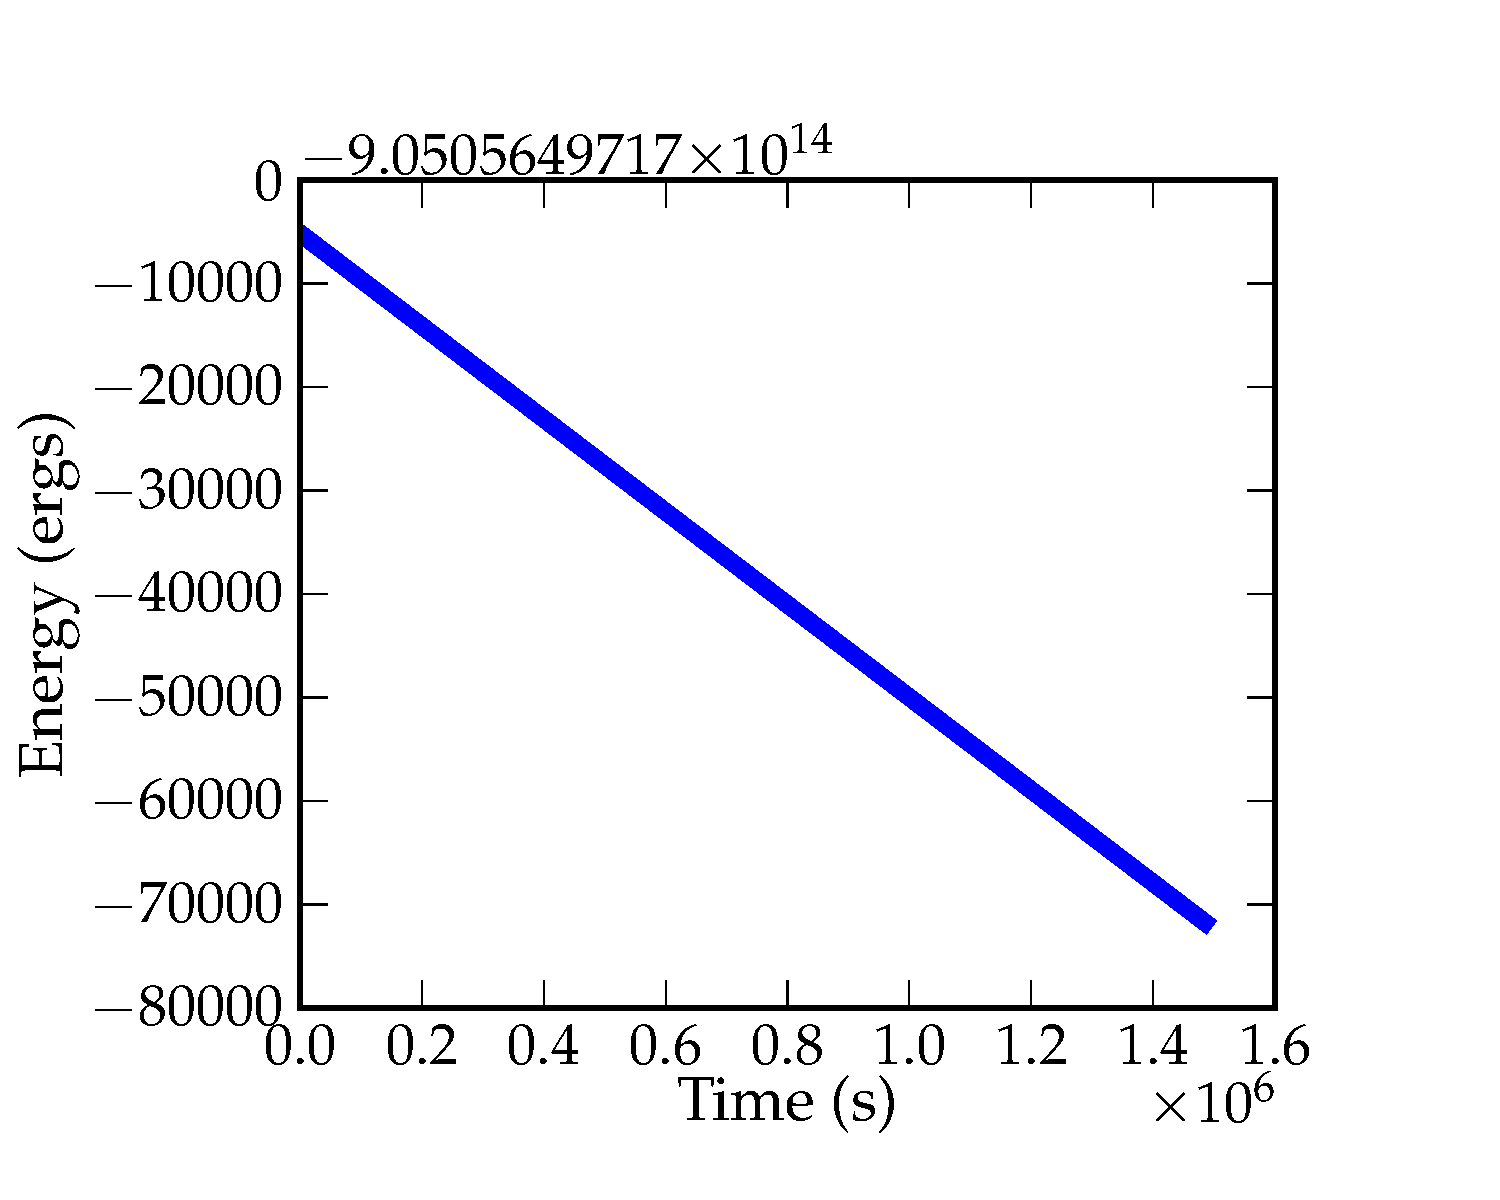
\includegraphics[width=0.5\textwidth]{output4_figs/energy.pdf}
\caption{This is the plot of $E$ as a function of time.}
\label{fig:simpleplot2}
\end{figure}

\begin{figure}[bth]
\centering
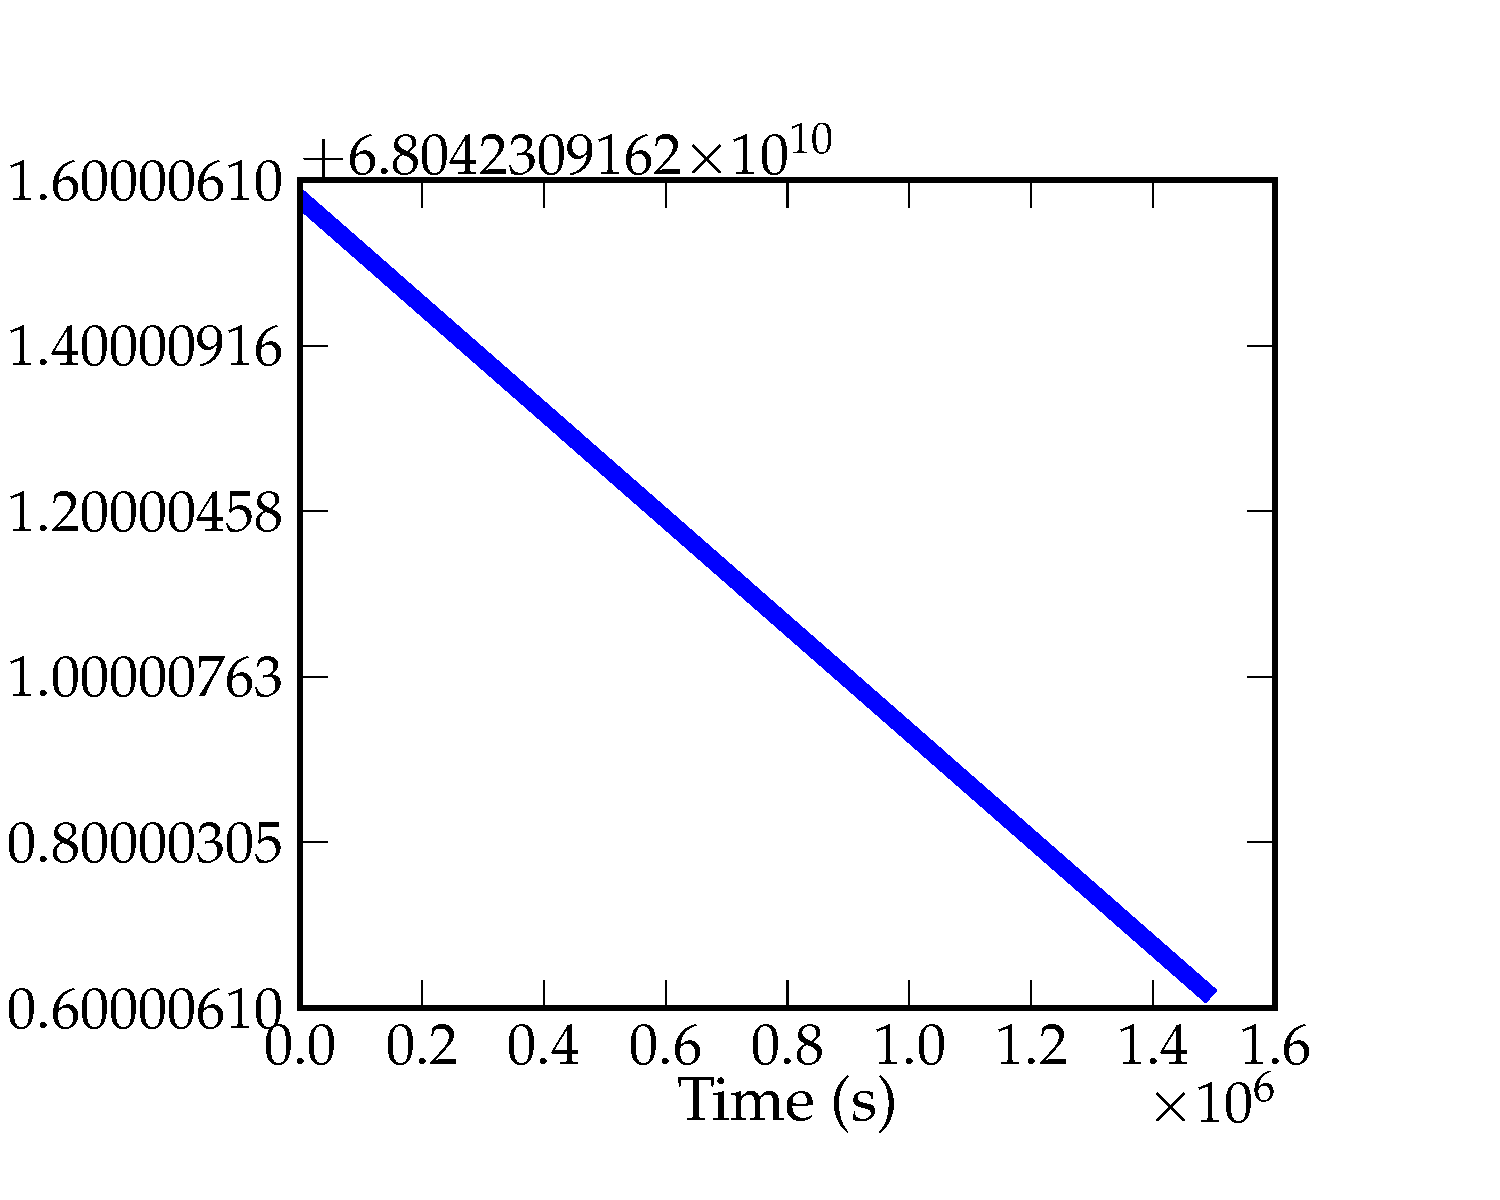
\includegraphics[width=0.5\textwidth]{output4_figs/angular_momentum.pdf}
\caption{This is the plot of $L_z$ as a function of time. This is in reduced units; to get to the actual value of $L_z$, multiply by $10^7$.}
\label{fig:simpleplot2}
\end{figure}

\section{Conclusion}

\end{document}
